\documentclass[conference]{IEEEtran}
\IEEEoverridecommandlockouts
% The preceding line is only needed to identify funding in the first footnote. If that is unneeded, please comment it out.
\usepackage{cite}
\usepackage{amsmath,amssymb,amsfonts}

\usepackage{algorithmicx}
\usepackage{algorithm}
\usepackage{algpseudocode}

\algrenewcommand\algorithmicindent{10pt}%

\usepackage{graphicx}
\usepackage{textcomp}
\usepackage{xcolor}

\usepackage{hyperref}
\usepackage{pgfplotstable}
\pgfplotsset{compat=newest}
\usepackage{subcaption}
\usepackage{xspace}

% TODO: remove the following in the final
\usepackage{lipsum}  
\newcommand{\bfspart}{\textsc{BFS-Part}\xspace}

\begin{document}

\title{\bfspart: A Graph Partitioning Approach to Scalable, Approximate Mesh Partitioning on Distributed Architectures\\
{\footnotesize \textsuperscript{*}Note: Sub-titles are not captured in Xplore and
should not be used}
\thanks{Identify applicable funding agency here. If none, delete this.}
}

\author{\IEEEauthorblockN{1\textsuperscript{st} Given Name Surname}
\IEEEauthorblockA{\textit{dept. name of organization (of Aff.)} \\
\textit{name of organization (of Aff.)}\\
City, Country \\
email address or ORCID}
\and
\IEEEauthorblockN{2\textsuperscript{nd} Given Name Surname}
\IEEEauthorblockA{\textit{dept. name of organization (of Aff.)} \\
\textit{name of organization (of Aff.)}\\
City, Country \\
email address or ORCID}
\and
\IEEEauthorblockN{3\textsuperscript{rd} Given Name Surname}
\IEEEauthorblockA{\textit{dept. name of organization (of Aff.)} \\
\textit{name of organization (of Aff.)}\\
City, Country \\
email address or ORCID}
\and
\IEEEauthorblockN{4\textsuperscript{th} Given Name Surname}
\IEEEauthorblockA{\textit{dept. name of organization (of Aff.)} \\
\textit{name of organization (of Aff.)}\\
City, Country \\
email address or ORCID}
\and
\IEEEauthorblockN{5\textsuperscript{th} Given Name Surname}
\IEEEauthorblockA{\textit{dept. name of organization (of Aff.)} \\
\textit{name of organization (of Aff.)}\\
City, Country \\
email address or ORCID}
\and
\IEEEauthorblockN{6\textsuperscript{th} Given Name Surname}
\IEEEauthorblockA{\textit{dept. name of organization (of Aff.)} \\
\textit{name of organization (of Aff.)}\\
City, Country \\
email address or ORCID}
}

\maketitle

\begin{abstract}
    \textcolor{red}{TODO}
\end{abstract}

\begin{IEEEkeywords}
keyword1, keyword2, keyword2
\end{IEEEkeywords}

\section{Introduction}
Mesh partitioning is an important preliminary step in large scale computations on distributed memory architectures. With the rise of new hardware on exascale computing, large scale computations are mostly implemented on supercomputers and server farms with distributed compute nodes. Optimal work distribution and load balancing of the mesh geometry is critical to achieve the best possible peak performance and scalability of such implementations. Mesh partitioning has been a well studied topic in the literature in the past decades. Mesh partitioning mainly focuses on optimizing two main objectives: (1) balanced number of elements/nodes in each partition, and (2) minimizing the number of boundary elements/nodes. One common method is to convert mesh element connectivity information into a graph data structure and employ a graph partitioning method to obtain mesh partitions. However, it is well known that the graph partitioning problem is an NP-Hard problem \cite{npcmpleteness}. This inherently makes obtaining optimal solution to mesh partitioning difficult. Therefore, most of the previous work on mesh partitioning rely on heuristics. On distributed architectures where the input mesh is already distributed, computing a new optimal mesh partitioning can be costly due to the communication overhead among distributed processes. If not carefully handled, parallel scalability of a distributed mesh partitioning algorithm can be significantly reduced due to communication and synchronization cost surpassing the local computations in the algorithm. 
\par
According to the used heuristics, mesh partitioning methods fall in to two main categories. (1) spatial mesh partitioning, and (2) non-spatial mesh partitioning. 
\par
\textbf{\emph{Spatial mesh partitioning}} methods mainly use the geometry coordinate information of mesh elements to obtain the partitioning. Recursive bisection methods [\textcolor{red}{TODO}] use the simplest form of heuristics: finding an optimal hyperplane in the mesh geometry to recursively partition the mesh. Oftentimes this procedure involves sorting the coordinates of elements in each spatial dimensions. Another commonly used method is to fit a Space Filling Curve (SFC) to obtain a global ordering of elements to get a partitioning along the order. Mesh data that involve quadtree or octree structures, commonly use Z-order curve to perform mesh partitioning. Creating the SFC order simplifies to a global sorting operation among the distributed processes. Since parallel-distributed sorting is well studied aspect, these spatial methods are adapted to their parallel versions for parallel distributed architectures [\textcolor{red}{TODO}]. Although spatial mesh partitioning methods are fast and scalable in distributed architectures, they do not explicitly consider the element connectivity information. Therefore, the partition quality of spatial partitioning is often worse than non-spatial methods. Especially when the mesh has a complex geometry with concave shapes, spatial partitioning methods produce partitions with very weak locality among elements inside each partition.


\section{Preliminaries}
\textcolor{red}{TODO}


\section{Methodology}
In this section we outline the data structures and key routines for \bfspart.


\subsection{Data Structures}
Similar to other mesh partitioning algorithms based on graphs, \bfspart algorithm requires the mesh element connectivity to be presented as a distributed graph data structure. We adhere to commonly used distributed CSR graph encoding as the graph input format to the algorithm. Apart from the graph adjacency structure, the only other data structures needed inside \bfspart are, the \verb|bfs_vec| and the \verb|scatter_map|.
\par
In each process, \verb|bfs_vec| is the vector to store the BFS status of each local vertex and each ghost vertex. \verb|bfs_vec| follows to the initial indexing of the vertices provided by the user. Each entry in the \verb|bfs_vec| contains two fields: 
\begin{enumerate}
    \item \verb|label| = Assigned new partition label
    \item \verb|distance| = Distance from the seed of the current assigned partition
\end{enumerate}
\par
Initially \verb|label| is set as \verb|NO_LABEL| implying the vertex is not visited by BFS. In each process, BFS vector entries corresponding to the ghost vertices are kept at one contiguous section in the \verb|bfs_vec|, referred to as the ``ghost portion''. Ghost portion of the BFS vector is partitioned according to the owning processes of ghost vertices. Thus, the ghost portion of the BFS vector is directly used as the ghost receive buffer for subsequent synchronization in BFS rounds. Each process maintains a \verb|scatter_map| for sending updated values to ghost processes. The \verb|scatter_map| in each process is created only once and repeatedly used for the communication in the BFS process.

% TODO: add BFS vector illustration with ghost portion and scatter map

\subsection{Algorithm}
Given the data structures, high level outline of \bfspart algorithm is given in Fig. \ref{algo:bfs-par-outline}. \bfspart requires some initial distribution of the graph across distributed processes. The initial distribution in each process needs to have some spatial locality in the graph vertices. Therefore, a spatial ordering type (e.g. Space Filling Curve) partitioning of the input mesh is ideal for the initial distribution. In an adaptive mesh/graph scenario, the initial partitioning can also be the previous partitioning before the refinement. 
\par
If the graph needs to be partitioned to $p$ parts, we assume the graph is initially distributed across $p$ processes. In each process, a vertex is picked as the local BFS \emph{seed}. Since the mesh/graph is initially partitioned according to some spatial ordering, we take the \emph{middle} (in the spatial order) vertex in each process as the \emph{seed} in that process. Each \emph{i}th \emph{seed} $(i \in [0, p-1])$ at process $i$ starts $i$th BFS exploring the graph structure in a BFS pattern. When exploring the graph, the BFS vector entry of each visited vertex is populated as \verb|label|=$i$ and \verb|distance|=\emph{graph distance from seed i}. If any $i$th BFS encounters an already visited vertex, the following takes place. If the current \verb|distance| value of the vertex is greater than the distance from $i$th seed, it is re-visited by $i$th BFS and updates its \verb|distance| and \verb|label| fields. Otherwise, that vertex is not re-visited by $i$th BFS. This process continues until there is no change to the BFS vector globally. In this way, each vertex gets their \verb|label| based on the closest seed. The \verb|label| field is the assignment in the final partitioning.
\par
The implementation is done using two main procedures. \textsc{BFS-Round()} and \textsc{Update-Ghost()} procedures are repeatedly applied until the global BFS state is stable across all processes. \textsc{Update-Ghost()} uses the pre-computed \verb|scatter_map| to prepare the sending buffer. BFS vector is updated with the received ghost values accordingly. Subsequent element/graph redistribution is done by accessing the computed \verb|distance| field in the BFS vector.

\begin{figure}  
    \begin{algorithmic}[1]  
    \Procedure{BFS-Partition}{$local\_graph$}  
    \State $bfs\_vec \gets$ Vector(size: $local\_graph.vertex\_count$)
    \State $seed \gets (local\_graph.own\_vertex\_count) /2$
    \State $bfs\_vec[seed].label \gets $ MPI\_rank
    \State $bfs\_vec[seed].distance \gets 0$
    \State $global \gets $ true
    \While{$global$}
        \State $global \gets $ false
        \State {$local \gets $ \Call{BFS-Round}{$local\_graph$, $bfs\_vec$}}
        \State \Call{Update-Ghost}{}()
        \State $global \gets$ \Call{MPI-Reduce}{$local$, LOGICAL\_OR}
    \EndWhile
    \State \textbf{return} $bfs\_vec$
    
    \EndProcedure  
    \end{algorithmic}

    \vspace{10pt}

    \begin{algorithmic}[1]  
    % \Procedure{BFS-Initial}{$local\_graph$, $bfs\_vec$}
    
    % \State $mid \gets (local\_graph.own\_vertex\_count) /2$
    % \State \Comment{\emph{SFC mid as the seed}}
    % \State $dist \gets 0$
    % \State $bfs\_vec[mid].label \gets $ MPI\_rank
    % \State $bfs\_vec[mid].distance \gets dist$
    % \State $bfs\_q \gets $ Queue()
    % \State $bfs\_q.enqueue(mid)$
    % \While {$bfs\_q \neq \emptyset$ }
    %     \State $dist = dist + 1$
    %     \State $v \gets bfs\_q.dequeue()$
    %     \ForAll{$u \in local\_graph.neighbors(v)$}
    %         \If{$bfs\_vec[u].label == $ NO\_LABEL}
    %             \State $bfs\_vec[u].label \gets $ MPI\_rank
    %             \State $bfs\_vec[u].distance \gets dist$
    %             \State $bfs\_q.enqueue(u)$
    %         \EndIf
    %     \EndFor

    % \EndWhile

    % \EndProcedure  

    \vspace{10pt}


    \Procedure{BFS-Round}{$local\_graph$, $bfs\_vec$}
    \State $changed \gets $ false
    \State $not\_stable \gets $ true

    \While{$not\_stable$}
        \State $not\_stable \gets $ false
        
        \State $bfs\_vec\_temp \gets bfs\_vec$.copy()
        \ForAll{$v \in local\_graph.vertices$}
        \State $best\_dist \gets bfs\_vec[v].distance$
        \State $best\_label \gets bfs\_vec[v].label$ 
            \ForAll{$u \in local\_graph.neighbors(v)$}
            \If{$best\_label ==$ NO\_LABEL \textbf{or} ($bfs\_vec[u].label \neq$ NO\_LABEL \textbf{and} $best\_dist > bfs\_vec[u].distance + 1 $)}
                \State $best\_dist \gets bfs\_vec[u].distance + 1$
                \State $best\_label \gets bfs\_vec[u].label$
                \State $not\_stable \gets $ true
                \State $changed \gets $ true

            \EndIf
            \EndFor
        \State $bfs\_vec\_temp[v].distance \gets best\_dist$
        \State $bfs\_vec\_temp[v].label \gets best\_label$

        \EndFor
        \State $bfs\_vec \gets bfs\_vec\_temp$
    \EndWhile
    \State \textbf{return} $changed$
    \EndProcedure


    \end{algorithmic}  
    \caption{\bfspart algorithm outline}  
    \label{algo:bfs-par-outline}  
\end{figure}

\subsection{Optimizations}
In \textsc{BFS-Round()} procedure, each \verb|while| loop iteration evaluates all the vertices and their neighborhoods. Since BFS flows similar to a frontier in the graph, it is sufficient to check and update the neighborhoods of the last updated vertices. To implement this, \textsc{Update-Ghost()} is modified to return the list of vertices that were updated in the last ghost value exchange. Thereafter, \textsc{BFS-Round()} proceeds to check only the neighborhood vertices of the last updated vertices. Furthermore, \textsc{Update-Ghost()} is optimized to compare the current send buffer with the previous send buffer to send only the updated values.

% \subsection{A list}
% \begin{itemize}
% \item \lipsum[1][1]
% \item \lipsum[1][1]
% \item \lipsum[1][1]
% \end{itemize}

% \subsection{Equations}

% \begin{equation}
% a+b=\gamma\label{eq}
% \end{equation}

% Be sure that the 
% symbols in your equation have been defined before or immediately following 
% the equation. Use ``\eqref{eq}'', not ``Eq.~\eqref{eq}'' or ``equation \eqref{eq}'', except at 
% the beginning of a sentence: ``Equation \eqref{eq} is . . .''

% \subsection{\LaTeX-Specific Advice}

% Please use ``soft'' (e.g., \verb|\eqref{Eq}|) cross references instead
% of ``hard'' references (e.g., \verb|(1)|). That will make it possible
% to combine sections, add equations, or change the order of figures or
% citations without having to go through the file line by line.

% Please don't use the \verb|{eqnarray}| equation environment. Use
% \verb|{align}| or \verb|{IEEEeqnarray}| instead. The \verb|{eqnarray}|
% environment leaves unsightly spaces around relation symbols.

% Please note that the \verb|{subequations}| environment in {\LaTeX}
% will increment the main equation counter even when there are no
% equation numbers displayed. If you forget that, you might write an
% article in which the equation numbers skip from (17) to (20), causing
% the copy editors to wonder if you've discovered a new method of
% counting.




% \subsection{Figures and Tables}
% \paragraph{Positioning Figures and Tables} Place figures and tables at the top and 
% bottom of columns. Avoid placing them in the middle of columns. Large 
% figures and tables may span across both columns. Figure captions should be 
% below the figures; table heads should appear above the tables. Insert 
% figures and tables after they are cited in the text. Use the abbreviation 
% ``Fig. \ref{fig}'', even at the beginning of a sentence.

% \begin{table}[htbp]
% \caption{Table Type Styles}
% \begin{center}
% \begin{tabular}{|c|c|c|c|}
% \hline
% \textbf{Table}&\multicolumn{3}{|c|}{\textbf{Table Column Head}} \\
% \cline{2-4} 
% \textbf{Head} & \textbf{\textit{Table column subhead}}& \textbf{\textit{Subhead}}& \textbf{\textit{Subhead}} \\
% \hline
% copy& More table copy$^{\mathrm{a}}$& &  \\
% \hline
% \multicolumn{4}{l}{$^{\mathrm{a}}$Sample of a Table footnote.}
% \end{tabular}
% \label{tab1}
% \end{center}
% \end{table}

% \begin{figure}[htbp]
% \centerline{
\includegraphics{figures/fig1.png}}
% \caption{Example of a figure caption.}
% \label{fig}
% \end{figure}

\section{Experimental Results}
We present experimental results for two aspects of the partitioning algorithm: (1) scalability and performance, and (2) partition quality. We compare our results with two other commonly used mesh partitioning schemes: parMETIS and PT-Scotch. We also consider the initial spatial ordered partitioning for evaluating the partition quality. All the tests are run on a collection of mesh files. Elements (tet or hex) in each mesh first are partitioned using the three different partitioning schemes. Further experiments on partition quality are performed on the new partition labels on elements.


\subsection{Input Files}
We used 3D mesh file collection from \cite{meshes}. Each mesh file in the collection contains either hexahedra or tetrahedra elements. We present experiment results for 50 meshes. Figures are presented for a set of selected 10 mesh files.


\subsection{Hardware Setup}
\textcolor{red}{\textcolor{red}{TODO}: extracted from HyMV paper, rephrase if needed.}

All experiments reported in this paper were performed on TACC's Frontera \cite{Frontera} supercomputer. Frontera is an Intel supercomputer at Texas Advanced Computing Center (TACC) with a total of 8,008 nodes, each consisting of a Xeon Platinum 8280 (“Cascade Lake”) processor, with a total of 448,448 cores. Each node has 192 GB of memory. The interconnect is based on Mellanox HDR technology with full HDR (200 Gb/s) connectivity between the switches and HDR100 (100 Gb/s) connectivity to compute nodes. In all experiments we bind each MPI process to each CPU core. We do not use OpenMP parallelism in the experiments.

\subsection{Scalability and Performance}
Since \bfspart is mostly a local operation, it is highly scalable in distributed memory environment. Furthermore, the number of rounds needed for \bfspart convergence (until BFS global stability is reached) is observed to be nearly constant regardless of the number of required partitions. These two observations contribute to the scalability of \bfspart. All 3 methods: \bfspart, parMETIS and PT-Scotch require the mesh as a distributed graph structure. Initial distribution was obtained using SFC partitioning. Fig \textcolor{red}{TODO} shows strong scalability results with selected 10 mesh files. Graph setup time and subsequent re-distribution time are omitted since those values are similar across all three methods in the comparison. While both parMETIS and PT-Scotch fail to achieve reasonable scalability, \bfspart shows near linear scalability for sufficiently larger input meshes. Although \bfspart shows sub-par scalability for smaller meshes, performance is consistently better than partMETIS and PT-Scotch, by a factor of 10 and 100 respectively.


\subsection{Partition Quality}



A high quality partitioning implies the partitions are balanced, and partition boundaries are minimal and \emph{smooth}. To provide a better intuition, we present a visualization of the partitioning. Fig. \ref{fig:tet-mesh-12} and \ref{fig:hex-mesh-4} show the partitioning view for two mesh files, partitioned into 10 and 20 parts respectively. It is evident that \bfspart produces reasonably high quality partitions with strong vertex locality, compared to a spatial order partitioning. \bfspart partitions contain a slight imbalance. However, in the next sections we show that this imbalance is negligible when used with a distributed numerical computation on the partitioned mesh.

\begin{figure}[htbp]
    \centering
    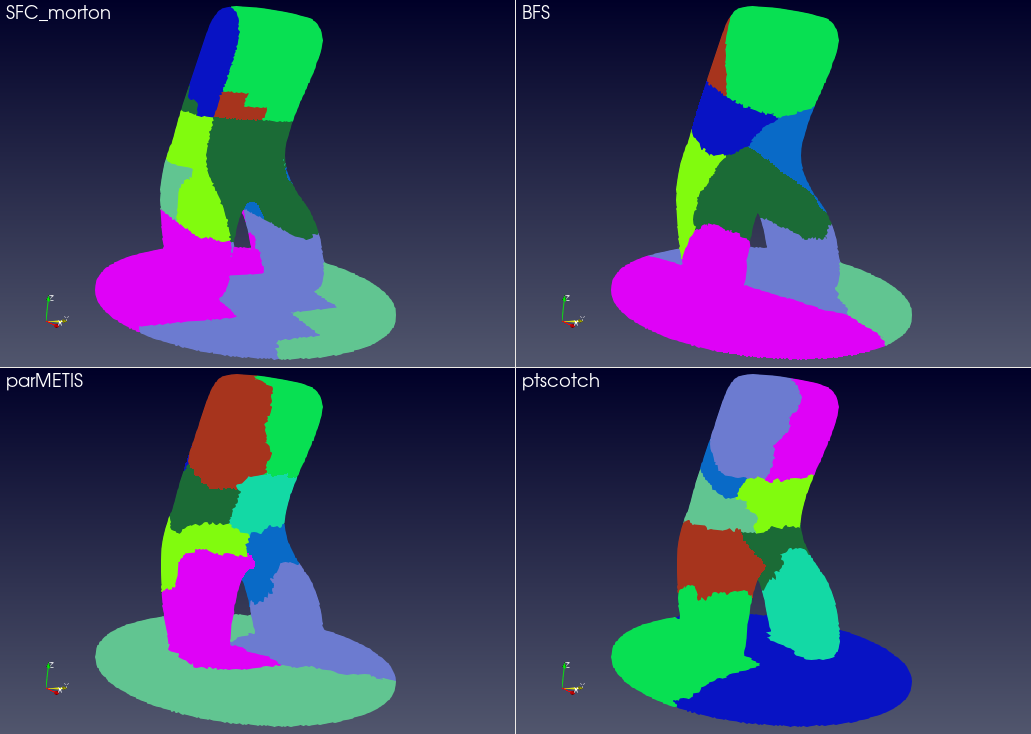
\includegraphics[width=\columnwidth]{figures/tet-mesh-12.png}
    \caption{Tet mesh partition view}
    \label{fig:tet-mesh-12}
\end{figure}

\begin{figure}[htbp]
    \centering
    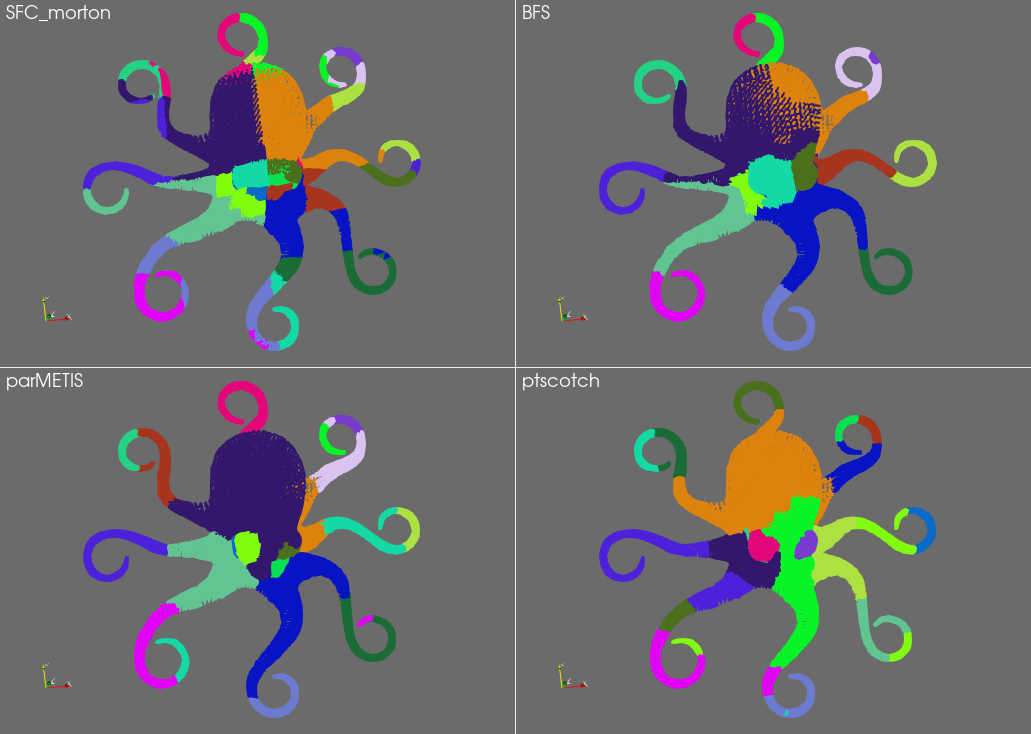
\includegraphics[width=\columnwidth]{figures/hex-mesh-4.png}
    \caption{Hex mesh partition view}
    \label{fig:hex-mesh-4}
\end{figure}

We further quantitatively compare the partition quality of the different methods using the following criteria
\begin{itemize}
    \item number of boundary elements in each new partition 
    \item $\lambda = $ ratio of total number of boundary elements to all elements
    \item $\rho_{max} = $ size of the largest partition size relative to ideal partition size
\end{itemize}



\begin{figure*}[htbp]
    \centering
    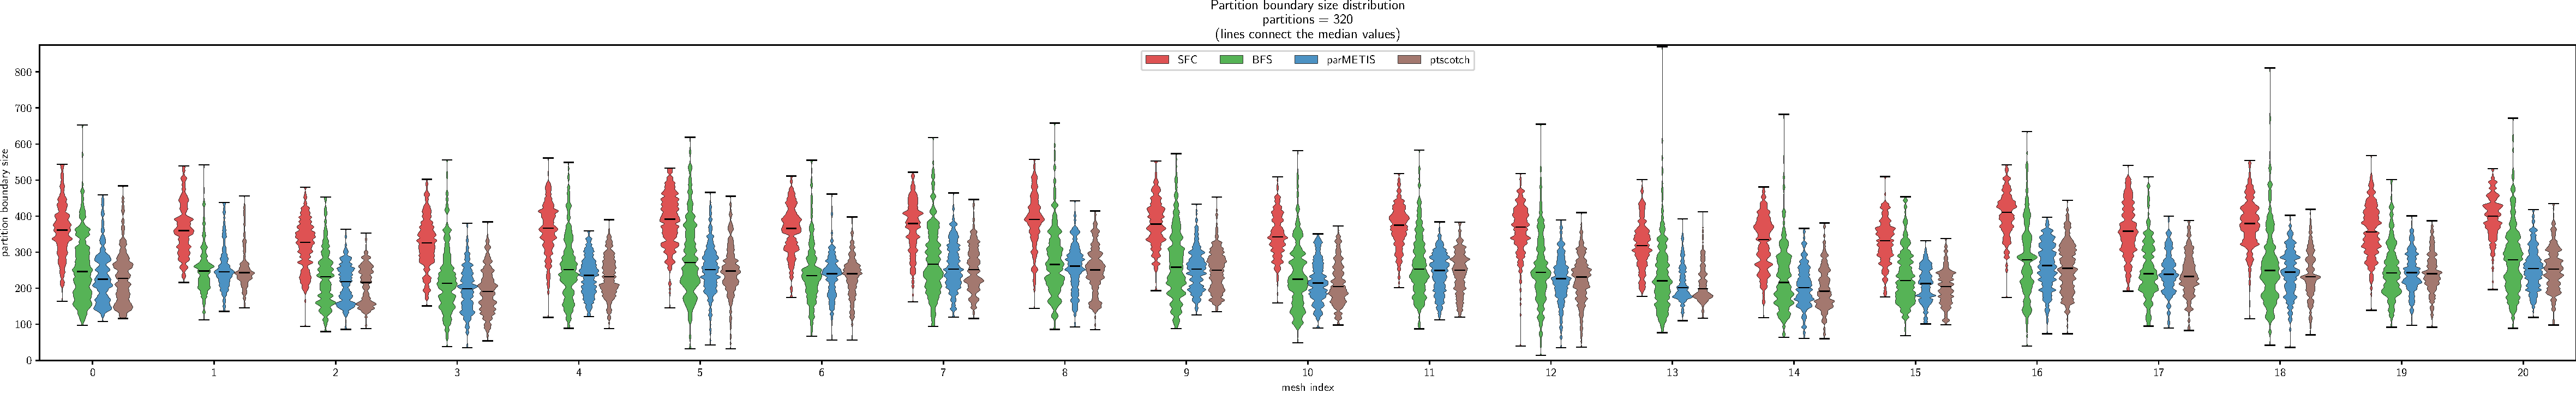
\includegraphics[width=\textwidth]{figures/boundary-sizes.pdf}
    \caption{Boundary Sizes Distribution}
    \label{fig:bdry-sizes}
\end{figure*}



Fig. \textcolor{red}{TODO} shows the distribution of the boundary size of each partition. \bfspart boundary size distribution is significantly better than the initial SFC partitioning. Since \bfspart is a local operation, we do not expect the quality of \bfspart partitions to be better than parMETIS or PT-Scotch. However, the median boundary size of \bfspart partitions is comparable with parMETIS and PT-Scotch. As observed in the Fig. \textcolor{red}{TODO}, it is possible to contain some high outliers in the boundary size distribution in \bfspart. However, in the next experiments we show that these outliers are negligible when the new partitioning is used with a large scale distributed computation on the mesh. Fig. \textcolor{red}{TODO} shows $\lambda$ for the all four partitioning methods. \bfspart consistently maintains $\lambda$ close to parMETIS and PT-Scotch. Fig. \textcolor{red}{TODO} presents $\rho$ for all partitioning methods. Since \bfspart relies on graph distance for partition assignment, there is no explicit control or constraint of the partition sizes. Therefore, the spread of the partition size distribution in \bfspart is wider than all other three methods. However, $\rho$ in \bfspart is consistently within 2-3 range. On a graph partitioning point of view, this imbalance is not optimal. However, in most very large scale numerical computations that involve distributed mesh partitioning, improvements in the boundary size can compensate for a slight imbalance in partition size. When such computations are scaled up for very large number of distributed processes, network communication often hinders the strong scalability. Communication cost is directly proportional to the boundary size of the partitions. Therefore, any significant improvement in boundary quality can improve the strong scalability. In most cases improvement of the communication can compensate for the local extra work caused by a slight imbalance in the partitions. In the next section we present empirical data to support this claim.


\subsection{Linear Solver Test}
We present a sparse linear solver test to show that the new partitions produced by \bfspart provide a significant performance benefit on subsequent distributed computations on partitioned mesh. Since we use mesh files as inputs, we use a linear solver on top of FEM like model on the nodes of the input mesh. After partitioning the 3D elements, nodes of each element are also assigned to partitions as follows. If a node is contained in only one element, node's partition is same as that element's partition. Otherwise, out of all the partitions of all the containing elements, the least numbered partition is considered as the node's partition. After node partitioning, elemental matrices are created with some dummy scalar values to assemble the global sparse matrix. We use PETSc \cite{petsc-web-page} for global matrix assembly and linear solver. Fig. \textcolor{red}{TODO} shows the time taken for PETSc GMRES \cite{GMRES} iterative solver with different partitioning schemes. Results show that the initial spatial ordering (SFC) partitioning is \emph{bad}, and it results in very poor scalability in the numerical solver. \bfspart gives a significant performance boost to the numerical solver, comparable with parMETIS and PT-Scotch. This experiment shows that a significant improvement in partition boundary quality in the \bfspart can overcome the slight imbalance in the partition sizes. When the linear solver is scaled-up to higher number of processes, the effect of communication overhead nullifies the effect of slight partition imbalance. 

\section{Conclusion}
This work presents a scalable, approximate mesh partitioning method using the Breadth First Search (BFS) graph algorithm. \bfspart is ideal for cases where the mesh has some initial partitioning (either from a spatial ordering or a previous partitioning before a mesh refinement). Since \bfspart mostly contain local computation and minimal point to point communication, it shows superior performance compared to two common partitioning schemes: parMETIS and PT-Scotch. Despite the considerable advantage in performance, \bfspart produces reasonably high quality partitions, comparable to parMETIS and PT-Scotch. Although \bfspart produces slightly imbalanced partitions, we show that the improvement in partition boundaries compensates for the imbalance. The linear solver test show that partitions obtained from \bfspart enables subsequent distributed numerical computations to sustain extreme scalability, similar to parMETIS and PT-Scotch partitions. 


\section*{Acknowledgment}

The authors acknowledge the Texas Advanced Computing Center (TACC) at The University of Texas at Austin for providing computational resources that have contributed to the research results reported within this paper. URL: \url{http://www.tacc.utexas.edu}
% \section*{References}


\bibliographystyle{IEEEtran}
\bibliography{IEEEabrv,main-bib.bib}

\vspace{12pt}
\textcolor{red}{IEEE conference templates contain guidance text for composing and formatting conference papers. Please ensure that all template text is removed from your conference paper prior to submission to the conference. Failure to remove the template text from your paper may result in your paper not being published.\\TODO: remove usepackage{lipsum} in the final}


\begin{figure*}
\pgfplotstabletypeset[
    col sep=comma,
    every head row/.style={
        before row={
        \hline 
            &  &  & \multicolumn{2}{c}{SFC} & \multicolumn{2}{c}{\bfspart} & \multicolumn{2}{c}{parMETIS} & \multicolumn{2}{c}{PT-Scotch} \\ },
            after row=\hline          
        },
    every column/.style={fixed, fixed zerofill, precision=2},
    columns/mesh/.style={column name=Mesh, fixed, precision=0},
    columns/n/.style={column name=$n$, precision=1, sci, precision=1},
    columns/p/.style={column name=$p$, fixed, precision=0},
    columns/sfc_lambda/.style={column name=$\lambda$},
    columns/sfc_rho_max/.style={column name=$\rho$},
    columns/bfs_lambda/.style={column name=$\lambda$},
    columns/bfs_rho_max/.style={column name=$\rho$},
    columns/parmetis_lambda/.style={column name=$\lambda$},
    columns/parmetis_rho_max/.style={column name=$\rho$},
    columns/ptscotch_lambda/.style={column name=$\lambda$},
    columns/ptscotch_rho_max/.style={column name=$\rho$},
    every last row/.style={after row=\hline}
]{data/part-quality.csv}
\end{figure*}
\end{document}
